\section{Některé další možnosti}


V tomto odstavci \orig{23} krátce naznačíme řešení speciálních
problémů, kterých jsme se dotkli v odst. 3.1 a 3.2.

\subsection{Poznámky k výpočtu funkcí vyrovnaných veličin při
  vyrovnání zprostředkujících pozorování}

V odst. 3.1 jsme definovali obecné funkce vyrovnaných veličin rovnicí

\noindent
\begin{align*}
\tag{3.39}  g = A_gv + B_gx + d,
\end{align*}

\noindent
kde $A_g$ $(p_g \times m)$ je nenulová matice. Naznačíme dva možné
způsoby zpracování funkcí (3.39) ortogonalizačním algoritmem. První
z nich je založen na převodu obecných funkcí (3.39) na zvláštní
případ (3.2), druhý vychází ze zobecněné ortogonalizace matice
(3.19), vhodně doplněné. U obou způsobů předpokládáme, že váhy
pozorovaných hodnot jsou dány diagonální maticí $P$.


Dosazením ze (3.1) do (3.39) dostaneme
%
\begin{align*}\tag{3.40}
  %
  g = A_gA_x + B_gx + A_gl + d = \bar{B}_gx + \bar{d}.
  %
\end{align*}
%
Vidíme tedy, že místo obecných funkcí (3.39) postačí uvažovat funkce
jednoduššího tvaru (3.2), kde matice $B_g$ a $d$ byly nahrazeny
maticemi
%
\begin{align*}\tag{3.41}
  \bar{B}_g = A_gA + B_g, \qquad \bar{d} = A_gl + d.
\end{align*}
%


Pokud bychom se chtěli vyhnout úpravám (3.41), můžeme hledané funkční
hodnoty i váhové koeficienty najít prostřednictvím submatic $W_{ij}$
$(i,j=1,2,3)$ získaných zobecněnou ortogonalizací, např. podle
schematu
%
\settowidth{\BMdx}{~$P^{-\frac{1}{2}}A^T_g$~}
\settowidth{\BMdy}{1cm}
\begin{align*}
  A_0 &= \tag{3.42}
    \vcenter{\hbox{
    \begin{tikzpicture}[x=\BMdx, y=\BMdy]
      \draw(0,3) -- (3,3); % rows
      \draw(0,2) -- (3,2);
      \draw(0,1) -- (3,1);
      \draw(0,0) -- (3,0);
      %
      \draw(0,0) -- (0,3); % cols
      \draw(1,0) -- (1,3);
      \draw(2,0) -- (2,3);
      \draw(3,0) -- (3,3);
      %
      \draw[thick] (0,2) rectangle (1,3);
      %
      \draw(0.5,2.5) node{$P^{-\frac{1}{2}}A$};
      \draw(1.5,2.5) node{$P^{-\frac{1}{2}}l$};
      \draw(2.5,2.5) node{$P^{-\frac{1}{2}}A^T_g$};
      %
      \draw(0.5,1.5) node{$E$};
      \draw(1.5,1.5) node{$0$};
      \draw(2.5,1.5) node{$0$};
      %
      \draw(0.5,0.5\BMdy) node{$B_g$};
      \draw(1.5,0.5\BMdy) node{$d$};
      \draw(2.5,0.5\BMdy) node{$0$};
      %
    \end{tikzpicture} }}
    \quad\longrightarrow\quad
    %
    \settowidth{\BMdx}{~$W_{22}$~}
    %\settowidth{\BMdy}{1cm}
    \vcenter{\hbox{
    \begin{tikzpicture}[x=\BMdx, y=\BMdy]
      \draw(0,3) -- (3,3); % rows
      \draw(0,2) -- (3,2);
      \draw(0,1) -- (3,1);
      \draw(0,0) -- (3,0);
      %
      \draw(0,0) -- (0,3); % cols
      \draw(1,0) -- (1,3);
      \draw(2,0) -- (2,3);
      \draw(3,0) -- (3,3);
      %
      \draw[thick] (0,2) rectangle (1,3);
      %
      \draw(0.5,2.5) node{$W_{11}$};
      \draw(1.5,2.5) node{$W_{12}$};
      \draw(2.5,2.5) node{$W_{13}$};
      %
      \draw(0.5,1.5) node{$W_{21}$};
      \draw(1.5,1.5) node{$W_{22}$};
      \draw(2.5,1.5) node{$W_{23}$};
      %
      \draw(0.5,0.5) node{$W_{31}$};
      \draw(1.5,0.5) node{$W_{32}$};
      \draw(2.5,0.5) node{$W_{33}$};
      %
    \end{tikzpicture} }}
    = W_0 \Punc{.}
\end{align*}



Analogickým postupem \orig{24} jako v odst. 3.1 se dá totiž dokázat,že
platí
%
\begin{align*}
\tag{3.43}  g     &= W_{32} + W^T_{13}W_{12}\\
\tag{3.44}  Q_{Lg} &= P^{-\frac{1}{2}}(W_{11}W^T_{31}
                   + \dot{A}^T_g  -W_{13})\\
\tag{3.45}  Q_{xg} &= W_{21}W^T_{31} - W_{23} \\
\tag{3.46}  Q_{gg} &= W_{31}W^T_{31} - (W_{33}+W^T_{33})
                   + (\dot{A}_g - W^T_{13})(\dot{A}_g - W^T_{13})^T,
\end{align*}
%
kde $\dot{A} = A_gP^{-\frac{1}{2}}$.


Vzorec (3.45), stejně jako postup při výpočtu matice $Q_{gg}$
naznačený v odst. 3.l, vycházejí z předpokladu, že matice $\dot{A}_g$
a $B_g$, byly zpracovány ortogonalizačním algoritmem. Věnujme nyní
pozornost otázce, jak najít váhové koeficienty funkcí formulovaných
dodatečně po vyřešení některé výchozí vyrovnávací úlohy, tedy tehdy,
když matice funkcí nebyly ortogonalizovány. Předpokládejme, že řešení
výchozí vyrovnávací úlohy bylo založeno na zobecněné ortogonalizaci
matice (3.19)

%
\settowidth{\BMdx}{~$P^{\frac{1}{2}}A$~}
\settowidth{\BMdy}{1cm}
\begin{align*}
\tag{3.47}
    \vcenter{\hbox{
    \begin{tikzpicture}[x=\BMdx, y=\BMdy]
      \draw(0,3) -- (2,3); % rows
      \draw(0,2) -- (2,2);
      \draw(0,1) -- (2,1);
      \draw(0,0) -- (2,0);
      %
      \draw(0,0) -- (0,3); % cols
      \draw(1,0) -- (1,3);
      \draw(2,0) -- (2,3);
      %
      \draw[thick] (0,2) rectangle (1,3);
      %
      \draw(0.5,2.5) node{$P^{\frac{1}{2}}A$};
      \draw(1.5,2.5) node{$P^{\frac{1}{2}}l$};
      %
      \draw(0.5,1.5) node{$E$};
      \draw(1.5,1.5) node{$0$};
      %
      \draw(0.5,0.5\BMdy) node{$B_g$};
      \draw(1.5,0.5\BMdy) node{$d$};
      %
    \end{tikzpicture} }}
    %
    \quad\longrightarrow\quad
    %
    \vcenter{\hbox{
    \begin{tikzpicture}[x=\BMdx, y=\BMdy]
      \draw(0,3) -- (2,3); % rows
      \draw(0,2) -- (2,2);
      \draw(0,1) -- (2,1);
      \draw(0,0) -- (2,0);
      %
      \draw(0,0) -- (0,3); % cols
      \draw(1,0) -- (1,3);
      \draw(2,0) -- (2,3);
      %
      \draw[thick] (0,2) rectangle (1,3);
      %
      \draw(0.5,2.5) node{$W_1$};
      \draw(1.5,2.5) node{$P^{\frac{1}{2}}v$};
      %
      \draw(0.5,1.5) node{$W_2$};
      \draw(1.5,1.5) node{$x$};
      %
      \draw(0.5,0.5\BMdy) node{$W_3$};
      \draw(1.5,0.5\BMdy) node{$g$};
      %
    \end{tikzpicture} }}
\end{align*}


Hledáme formuli pro výpočet matice $Q'_{gg}$ váhových koeficientů
funkcí
%
\begin{align*}
\tag{3.48}   g' = A'_gv + B'_gx + C'_gg + d'
\end{align*}

\noindent
pomocí veličin získaných při transformaci (3.47).
%
Označme $\dot{A}'_g = A'_gP^{-\frac{1}{2}}$. Ukazuje se, že potom platí
%
\begin{align*}
  \tag{3.49}
  Q'_{gg} =
  \begin{bmatrix}
    \dot{A}'_g & B'_g &  C'_g
  \end{bmatrix}
  \begin{bmatrix}
    W^{}_1W^T_1 & W^{}_1W^T_2 & W^{}_1W^T_3 \\
    W^{}_2W^T_1 & W^{}_2W^T_2 & W^{}_2W^T_3 \\
    W^{}_3W^T_1 & W^{}_3W^T_2 & W^{}_3W^T_3 \\
  \end{bmatrix}
  \begin{bmatrix}
    \dot{A}'_g & B'_g &  C'_g
  \end{bmatrix}^T
\end{align*}


\noindent nebo alternativně \orig{25}
%
\begin{align*}
  \tag{3.50} Q'_{gg} =
  (\dot{A}'W_1 + B'_{g}W_2 + C'_gW_3)
  (\dot{A}'W_1 + B'_{g}W_2 + C'_gW_3)^T.
\end{align*}



\subsection{Určení některých transformačních matic při vyrovnání
            zprostředkujících a podmínkových pozorování}

Transformačními maticemi $T$ budeme rozumět matice, umožňující
přímý převod absolutních členů v rovnicích oprav nebo
v podmínkových rovnicích na opravy, funkce vyrovnaných veličin a
příp. neznámé. Znalost takových matic je užitečná zejména tehdy,
máme-li vícenásobně opakovat vyrovnání některé úlohy s postupně
měněnými vektory absolutních členů, jako je tomu např. při
zpracování opakovaných měření v určité geodetické síti.
Pro jednoduchost budeme při odvození matic $T$ přejpokládat
jednotkové váhy pozorovaných hodnot.


\subsubsection*{A. Vyrovnání zprostředkujících pozorování}
\subsubsection*{A.1. Transformace $~l \rightarrow v$}

Podle (3.8) je
%
\begin{align*}
  \tag{3.51}  v= (E - WW^T)l = T_1l.
\end{align*}
%
Ze vzorce (2.21) vyplývá, že transformační matici
%
\begin{align*}
  \tag{3.52}  T_1 = E - WW^T
\end{align*}
%
můžeme najít zobecněnou ortogonalizací
%
\begin{align*}
\tag{3.53}
    \vcenter{\hbox{
    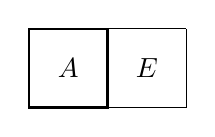
\begin{tikzpicture}[x=1cm, y=1cm]
      \draw(0,1) -- (2,1);
      \draw(0,0) -- (2,0);
      \draw(0,0) -- (0,1);
      \draw(1,0) -- (1,1);
      \draw(2,0) -- (2,1);
      %
      \draw[thick] (0,0) rectangle (1,1);
      %
      \draw(0.5,0.5) node{$A$};
      \draw(1.5,0.5) node{$E$};
      %
    \end{tikzpicture} }}
    \quad\longrightarrow\quad
    \vcenter{\hbox{
    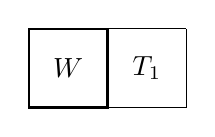
\begin{tikzpicture}[x=1cm, y=1cm]
      \draw(0,1) -- (2,1);
      \draw(0,0) -- (2,0);
      \draw(0,0) -- (0,1);
      \draw(1,0) -- (1,1);
      \draw(2,0) -- (2,1);
      %
      \draw[thick] (0,0) rectangle (1,1);
      %
      \draw(0.5,0.5) node{$W$};
      \draw(1.5,0.5) node{$T_1$};
      %
    \end{tikzpicture} }}
    %
\end{align*}
%


Poznamenejme, že symetrická matice $T_1$ má dvě zajímavé vlastnosti.
Předně platí
%
\begin{align*}
  \tag{3.54}   T_1A = (E - WW^T) = A - WR = 0.
\end{align*}
%
Dále je
\begin{align*}
  \tag{3.55}   T^2_1 = (E - WW^T - WW^T + WW^T) = T_1.
\end{align*}

\noindent
Matice se druhou \orig{26} uvedenou vlastností (3.95) se označují jako
idempotentní [47, str.~94].

Porovnáme-li (3.52) se vzorcem (3.10), dostaneme ještě vztah
mezi maticí $T_1$  a maticí váhových koeficientů $Q_{LL}$
%
\begin{align*}
  \tag{3.56}   T_1 = E - Q_{LL}.
\end{align*}




\subsubsection*{A.2. Transformace $~l \rightarrow x$}


Ze (3.7) bezprostředně vyplývá, že transformaci absolutních
členů na neznámé popisují vzorce
%
\begin{align*}
  \tag{3.57}   x = T_2l, \qquad T_2 = -R^{-1}W^T.
\end{align*}
%
Transformační matici $T_2$, je možno na základě (2.22) určit
zobecněnou ortogonalizací
%
\begin{align*}
  \tag{3.58}
    \vcenter{\hbox{
    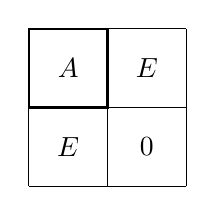
\begin{tikzpicture}[x=1cm, y=1cm]
      \draw(0,2) -- (2,2); % rows
      \draw(0,1) -- (2,1);
      \draw(0,0) -- (2,0);
      %
      \draw(0,0) -- (0,2); % cols
      \draw(1,0) -- (1,2);
      \draw(2,0) -- (2,2);
      %
      \draw[thick] (0,1) rectangle (1,2);     % top left cell
      %
      \draw(0.5,1.5) node{$A$};               % first row
      \draw(1.5,1.5) node{$E$};
      %%
      \draw(0.5,0.5) node{$E$};               % second row
      \draw(1.5,0.5) node{$0$};
      %
    \end{tikzpicture} }}
    \quad\longrightarrow\quad
    \vcenter{\hbox{
    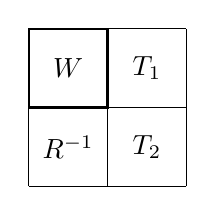
\begin{tikzpicture}[x=1cm, y=1cm]
      \draw(0,2) -- (2,2); % rows
      \draw(0,1) -- (2,1);
      \draw(0,0) -- (2,0);
      %
      \draw(0,0) -- (0,2); % cols
      \draw(1,0) -- (1,2);
      \draw(2,0) -- (2,2);
      %
      \draw[thick] (0,1) rectangle (1,2);     % top left cell
      %
      \draw(0.5,1.5) node{$W$};               % first row
      \draw(1.5,1.5) node{$T_1$};
      %%
      \draw(0.5,0.5) node{$R^{-1}$};          % second row
      \draw(1.5,0.5) node{$T_2$};
      %
    \end{tikzpicture} }}
    %
\end{align*}
%
Matice $T_2$ stejně jako matice $T_1$, má některé pozoruhodné
vlastnosti. Snadno se můžeme přesvědčit o tom, že platí
%
\begin{align*}
  \tag{3.59}  A(-T_2)A &= AR^{-1}W^TWR = A \\
  \tag{3.60}  (-T_2)A(-T_2) &= R^{-1}W^TWRR^{-1}W^T = -T_2\\
  \tag{3.61}  \left\{A(-T_2)\right\}^T &= (AR^{-1}W^T)^T
  = WW^T = AR^{-1}W^T = A(-T_2)\\
  \tag{3.62}  \left\{(-T_2)\right\}^T &= (R^{-1}W^TWR)^T = E
  = \left\{(-T_2)A\right\} \Punc{.}
\end{align*}

\noindent
Ze vztahů (3.59) až (3.62) vyplývá, že matice ($-T_2$) je
\name{MOOROVOU} [56] \emph{pseudoinverzní maticí} k matici $A$, neboť
splňuje všechny podmínky na tuto matici kladené [13,str.~77], [53].  Z
rovnosti (3.59) vyplývá, že matice ($-T_2$) představuje současně tzv.
zobecněnou inverzní matici k matici $A$ ve smyslu \name{BJERHAMMAROVĚ}
[48].  Vidíme tedy, že ortogonalizační algoritmus může být užit nejen
k řešení vyrovnávacích problémů, ale i při hledání pseudoinverzních
resp. zobecněných inverzních matic. Je třeba ovšem zdůraznit, že tomu
tak je pouze v případě, kdy sloupce matice $A$ jsou lineárně
nezávislé.

\subsubsection*{A.3. Transformace $~l\rightarrow g$\\
                funkce zjednodušeného tvaru (3.2)}

Podle (3.9) je \orig{27}
%
\begin{align*}
  \tag{3.63}   g - d = -B_gR^{-1}W^Tl = T_3l.
\end{align*}
%
Vyjdeme-li ze (2.22), můžeme transformační matici
\begin{align*}
  \tag{3.64} T_3 = -B_gR^{-1}W^T
\end{align*}
%
najít zobecněnou ortogonalizací
%
\begin{align*}
  \tag{3.65}
      \vcenter{\hbox{
    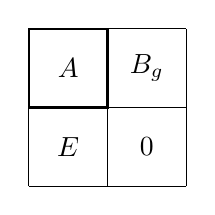
\begin{tikzpicture}[x=1cm, y=1cm]
      \draw(0,2) -- (2,2); % rows
      \draw(0,1) -- (2,1);
      \draw(0,0) -- (2,0);
      %
      \draw(0,0) -- (0,2); % cols
      \draw(1,0) -- (1,2);
      \draw(2,0) -- (2,2);
      %
      \draw[thick] (0,1) rectangle (1,2);     % top left cell
      %
      \draw(0.5,1.5) node{$A$};               % first row
      \draw(1.5,1.5) node{$B_g$};
      %%
      \draw(0.5,0.5) node{$E$};               % second row
      \draw(1.5,0.5) node{$0$};
      %
    \end{tikzpicture} }}
    \quad\longrightarrow\quad
    \vcenter{\hbox{
    \settowidth{\BMdx}{~$B_gR^{-1}$~}
    \settowidth{\BMdy}{1.0cm}
    \begin{tikzpicture}[x=\BMdx, y=\BMdy]
      \draw(0,2) -- (2,2); % rows
      \draw(0,1) -- (2,1);
      \draw(0,0) -- (2,0);
      %
      \draw(0,0) -- (0,2); % cols
      \draw(1,0) -- (1,2);
      \draw(2,0) -- (2,2);
      %
      \draw[thick] (0,1) rectangle (1,2);     % top left cell
      %
      \draw(0.5,1.5) node{$W$};               % first row
      \draw(1.5,1.5) node{$T_1$};
      %%
      \draw(0.5,0.5) node{$B_gR^{-1}$};          % second row
      \draw(1.5,0.5) node{$T_3$};
      %
    \end{tikzpicture} }} \Punc{.}
    %
\end{align*}


\subsubsection*{A.4. Transformace $~l \rightarrow g$\\
  funkce obecného tvaru (3.39)}

Dosazením ze (3.51) a (3.7) do (3.39) dostaneme
%
\begin{align*}
  \tag{3.66}   g -d = \left\{A_g(E - WW^T) - B_gR^{-1}W^T\right\}l
  = (T_4 + T'_3)l .
\end{align*}
%
Matici $T'_3$  lze najít analogicky jako jako matici $T_3$, ve (3.65).
Matici $T_4$ umožnuje určit zobecněná ortogonalizace
%
\begin{align*}
\tag{3.67}
    \vcenter{\hbox{
    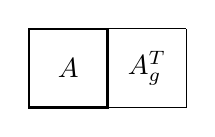
\begin{tikzpicture}[x=1cm, y=1cm]
      \draw(0,1) -- (2,1);
      \draw(0,0) -- (2,0);
      \draw(0,0) -- (0,1);
      \draw(1,0) -- (1,1);
      \draw(2,0) -- (2,1);
      %
      \draw[thick] (0,0) rectangle (1,1);
      %
      \draw(0.5,0.5) node{$A$};
      \draw(1.5,0.5) node{$A^T_g$};
      %
    \end{tikzpicture} }}
    \quad\longrightarrow\quad
    \vcenter{\hbox{
    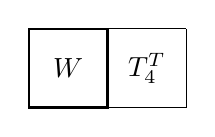
\begin{tikzpicture}[x=1cm, y=1cm]
      \draw(0,1) -- (2,1);
      \draw(0,0) -- (2,0);
      \draw(0,0) -- (0,1);
      \draw(1,0) -- (1,1);
      \draw(2,0) -- (2,1);
      %
      \draw[thick] (0,0) rectangle (1,1);
      %
      \draw(0.5,0.5) node{$W$};
      \draw(1.5,0.5) node{$T^T_4$};
      %
    \end{tikzpicture} }}
    %
\end{align*}
%
založená na (2.21).

\subsubsection*{B. Vyrovnání podmrínkových pozorování}
\subsubsection*{B.1. Transformace $~u^T \rightarrow v$}

Vyjdeme-li ze (3.29) můžeme psát
%
\begin{align*}
\tag{3.68}  v = -WR^{-T}u^T = T_5u^T,\quad T_5 = -ER^{-T}.
\end{align*}
%


Transformační matice $T_5$ může být opět nalezené zobecněnou
ortogonalizací vhodně definované matice. S uvážením (2.20) až
(2.22) bude schematicky
%
\begin{align*}
  \tag{3.69}
    \vcenter{\hbox{
    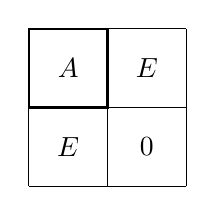
\begin{tikzpicture}[x=1cm, y=1cm]
      \draw(0,2) -- (2,2); % rows
      \draw(0,1) -- (2,1);
      \draw(0,0) -- (2,0);
      %
      \draw(0,0) -- (0,2); % cols
      \draw(1,0) -- (1,2);
      \draw(2,0) -- (2,2);
      %
      \draw[thick] (0,1) rectangle (1,2);     % top left cell
      %
      \draw(0.5,1.5) node{$A$};               % first row
      \draw(1.5,1.5) node{$E$};
      %%
      \draw(0.5,0.5) node{$E$};               % second row
      \draw(1.5,0.5) node{$0$};
      %
    \end{tikzpicture} }}
    \quad\longrightarrow\quad
    \vcenter{\hbox{
    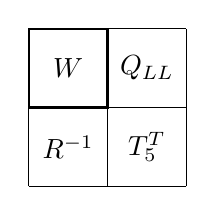
\begin{tikzpicture}[x=1cm, y=1cm]
      \draw(0,2) -- (2,2); % rows
      \draw(0,1) -- (2,1);
      \draw(0,0) -- (2,0);
      %
      \draw(0,0) -- (0,2); % cols
      \draw(1,0) -- (1,2);
      \draw(2,0) -- (2,2);
      %
      \draw[thick] (0,1) rectangle (1,2);     % top left cell
      %
      \draw(0.5,1.5) node{$W$};               % first row
      \draw(1.5,1.5) node{$Q_{LL}$};
      %%
      \draw(0.5,0.5) node{$R^{-1}$};          % second row
      \draw(1.5,0.5) node{$T^T_5$};
      %
    \end{tikzpicture} }}
    %
\end{align*}
%

\subsubsection*{B.1. Transformace $~u^T \rightarrow g^T$}

Dosazením \orig{28} ze (3.68) do (3.22) dostaneme
%
\begin{align*}
  \tag{3.70}
  g^T - d^T = -A^T_gWR^{-T}u^T = T_6u^T.
\end{align*}
%
Stejně jako všechny předcházející transformační matice, můžeme
i matici $T_6$ určit zobecněnou ortogonalizací, tentokrát
s užitím (2.22) podle schematu
%
\begin{align*}
  \tag{3.71}
    \vcenter{\hbox{
    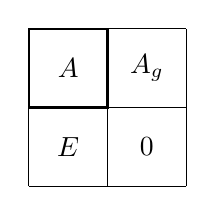
\begin{tikzpicture}[x=1cm, y=1cm]
      \draw(0,2) -- (2,2); % rows
      \draw(0,1) -- (2,1);
      \draw(0,0) -- (2,0);
      %
      \draw(0,0) -- (0,2); % cols
      \draw(1,0) -- (1,2);
      \draw(2,0) -- (2,2);
      %
      \draw[thick] (0,1) rectangle (1,2);     % top left cell
      %
      \draw(0.5,1.5) node{$A$};               % first row
      \draw(1.5,1.5) node{$A_g$};
      %%
      \draw(0.5,0.5) node{$E$};               % second row
      \draw(1.5,0.5) node{$0$};
      %
    \end{tikzpicture} }}
    \quad\longrightarrow\quad
    \vcenter{\hbox{
    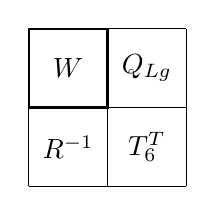
\begin{tikzpicture}[x=1cm, y=1cm]
      \draw(0,2) -- (2,2); % rows
      \draw(0,1) -- (2,1);
      \draw(0,0) -- (2,0);
      %
      \draw(0,0) -- (0,2); % cols
      \draw(1,0) -- (1,2);
      \draw(2,0) -- (2,2);
      %
      \draw[thick] (0,1) rectangle (1,2);     % top left cell
      %
      \draw(0.5,1.5) node{$W$};               % first row
      \draw(1.5,1.5) node{$Q_{Lg}$};
      %%
      \draw(0.5,0.5) node{$R^{-1}$};          % second row
      \draw(1.5,0.5) node{$T^T_6$};
      %
    \end{tikzpicture} }}.
    %
\end{align*}
%
